\documentclass[tikz,border=5pt]{standalone}
\usepackage{times}
\usepackage{amsmath,amssymb}
\usetikzlibrary{positioning,fit,arrows.meta,backgrounds,shapes.geometric,calc,shadows,decorations.pathreplacing}

\begin{document}
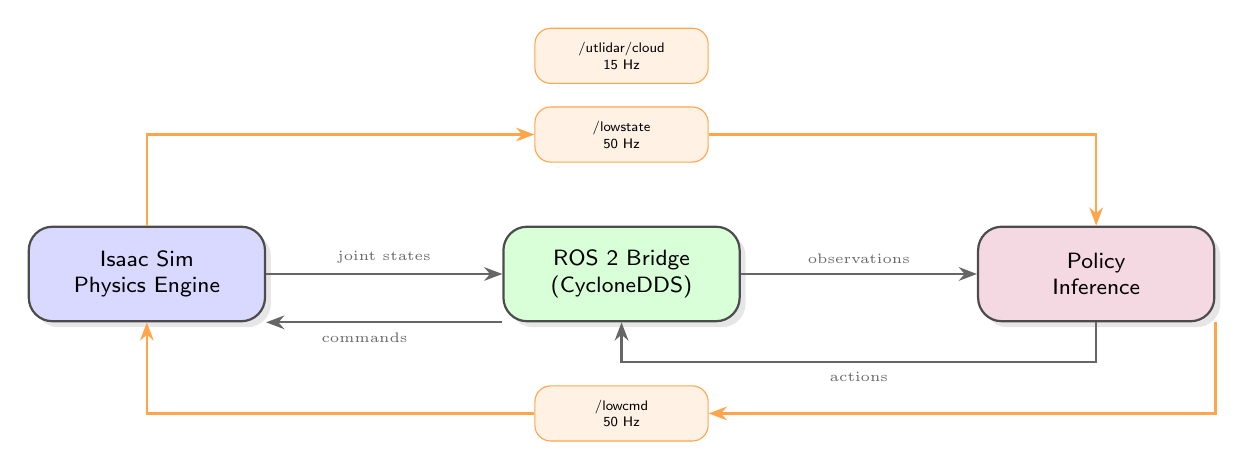
\begin{tikzpicture}[
    node distance=1cm and 2cm,
    component/.style={
        draw=black!70,
        rounded corners=3mm,
        minimum width=3cm,
        minimum height=1.2cm,
        font=\sffamily\footnotesize,
        fill=white,
        thick,
        align=center,
        drop shadow={opacity=0.2}
    },
    topic/.style={
        draw=orange!70,
        fill=orange!10,
        rounded corners=2mm,
        minimum width=2.2cm,
        minimum height=0.7cm,
        font=\sffamily\tiny,
        align=center
    },
    arrow/.style={->, >=Stealth, thick, color=black!60}
]

% Isaac Sim
\node[component, fill=blue!15] (sim) {Isaac Sim\\Physics Engine};

% ROS2 Bridge
\node[component, fill=green!15, right=3cm of sim] (bridge) {ROS 2 Bridge\\(CycloneDDS)};

% Policy Node
\node[component, fill=purple!15, right=3cm of bridge] (policy) {Policy\\Inference};

% Topics
\node[topic, above=0.8cm of bridge] (lowstate) {/lowstate\\50 Hz};
\node[topic, below=0.8cm of bridge] (lowcmd) {/lowcmd\\50 Hz};
\node[topic, above=1.8cm of bridge] (lidar) {/utlidar/cloud\\15 Hz};

% Arrows
\draw[arrow] (sim.east) -- node[above, font=\tiny] {joint states} (bridge.west);
\draw[arrow] (bridge.east) -- node[above, font=\tiny] {observations} (policy.west);
\draw[arrow] (policy.south) -- ++(0,-0.5) -| node[below, font=\tiny, pos=0.25] {actions} (bridge.south);
\draw[arrow] (bridge.south west) -- ++(-0.5,0) |- node[below, font=\tiny, pos=0.75] {commands} (sim.south east);

% Topic connections
\draw[arrow, orange!70] (sim.north) |- (lowstate.west);
\draw[arrow, orange!70] (lowstate.east) -| (policy.north);
\draw[arrow, orange!70] (policy.south east) |- (lowcmd.east);
\draw[arrow, orange!70] (lowcmd.west) -| (sim.south);

\end{tikzpicture}
\end{document}
